% siminos/spatiotemp/chapter/Ihara.tex
% $Author: predrag $ $Date: 2021-08-10 11:56:19 -0400 (Tue, 10 Aug 2021) $

% called by Ising.tex
\section{{Ihara} zeta functions}
\label{sect:Ihara}

%\newcommand{\Tr}{\mbox{\rm tr}\,}
\renewcommand{\Tr}{\mbox{Tr}\,}

\begin{description}

    \PCpost{2020-05-12}{.
\begin{itemize}
  \item
I think it should be little work to verify for \templatt\ that the Boss
determinant \refeq{gridZeta}, \refeq{Rangarajan2}, \refeq{Rangarajan2a}
for the Ihara zeta function (that counts undirected loops) is the Isola's
Bowen-Ruelle zeta \refeq{Ising:Isola90-13}.
This counts walks of the cat map directed Markov graph.
  \item
Clair's square 2D lattice \refeq{IharaGrid} presumably counts
1D loops (returning walks) on a 2D lattice. So does
Kasteleyn\rf{Kasteleyn63} elliptic integral of the first kind
\refeq{IsingZeta} (see also \refeq{Cserti00(38)}).
  \item
For \catlatt\ we count 2D tori (Bravais lattices); expect a variable
$z_j$ for every translational symmetry direction, not a single $z$ as in
\refeq{IsingZeta}. In Ising models, one counts the 2D configurations - so
how come Ihara functions can do that? Or can they?
  \item
Explain the relation between a discrete torus and the Cayley graph.
For example, given $n\in\naturals^*$, let $G_n$ denote the Cayley graph
$\left({{\integers}/{n\integers},\left\lbrace{\pm1}\right\rbrace}\right)$.
\end{itemize}
    }

\end{description}


\subsection{Heat equation}
\label{sect:heatEq}
    \PC{2020-03-15}{
I like Elaydi\rf{Elaydi05}'s Sect.~3.5.5 {\em The heat equation}
    }
Let $T_{n\zeit}$ be temperature at spatial site $n$ at time $\zeit$. The
heat equation for temperature field $\mathsf{T}=\{T_{n\zeit}\}$ is
\beq
\pde_\zeit \mathsf{T} = D\,\Laplacian_x \mathsf{T}
\,,
\ee{Elaydi05(3.5.22)}
where $D$ is the diffusion constant. Convert this into an integer lattice
difference equation over a finite spacetime domain by the same rescaling
as for \refeq{forwDer}.
Then the heat difference equation for temperature field
$\mathsf{T}=\{T_{n\zeit}\}$ over a finite tile $\LTS{}{}{}$ is
\beq
\pde_\zeit \mathsf{T} = \beta\,\Laplacian_x \mathsf{T}
\,,
\ee{Elaydi05(3.5.22)a}
In the space and time continuum limits, $\beta$ is related to the
diffusion constant by
\[
  \beta = \frac{\Delta\zeit}{(\Delta x)^2}{\diffCon}
        = \frac{\speriod{}^2}{\period{}}{\diffCon}
  \,.
\]


\subsection{Heat kernel}
\label{sect:heatKernel}

\begin{description}

    \PCpost{2020-05-05}{
Jorgenson and Lang\rf{JorLan01} {\em The ubiquitous heat kernel}
    }

    \PCpost{2020-05-13}{
For general regular graphs with a transitive group action,
in particular the discrete tori,  a zeta function
has been defined in an impressive paper by
Chinta, Jorgenson and Karlsson\rf{ChJoKa14} {\em Heat kernels on regular
graphs and generalized {Ihara} zeta function formulas}:
Let q be a positive integer and $G$ be a (q + 1)-regular graph. There is
an associated heat kernel $K_G(t, x_0, x)$ corresponding to the Laplacian
formed by considering the adjacency matrix on $G$. The building blocks of
$K_G$ are I-Bessel functions, and the number
of geodesics from a fixed base point $x_0$ to $x$ of length $m$.

$N^0_m$ denotes the number of closed geodesics of length $m$ in $G$ with
base point $x_0$.

They give a clear introduction into heat kernels on graphs, the origin
of I-Bessel functions, and the relationto the number of paths.
They also deduce the classical Ihara determinantal formula.

There is a second expression for the heat kernel coming from spectral
considerations. Equating the two expressions for the heat kernel, as in
known approaches to the Poisson summation formula or the Selberg trace
formula, one obtains an identity which is a type of theta inversion
formula. To this identity they apply an integral transform,
a Laplace transform with a change of variables, and
obtain the logarithmic derivative of the Ihara zeta function.

For finite graphs, the classical Ihara zeta function is their Ihara zeta
function raised to the power equaling the number of vertices (by fixing
the base point $x_0$, they can work with infinite graphs). They give a
formula, their Theorem 1.3, for $1/zeta$ as an integral over the spectral
measure for the Laplacian.

They also count geodesics paths, not only closed geodesics paths. That
corresponds to computing the Hurwitz zeta function instead of the Riemann
zeta function, they say.

    }

    \PCpost{2020-05-13}{
Chinta, Jorgenson and Karlsson\rf{ChJoKa10}
{\em Zeta functions, heat kernels, and spectral asymptotics on
degenerating families of discrete tori}:

By a discrete torus we mean the Cayley graph associated to a finite
product of finite cycle groups with the generating set given by choosing
a generator for each cyclic factor.

We examine the
spectral theory of the combinatorial Laplacian for sequences of discrete
tori when the orders of the cyclic factors tend to infinity at comparable
rates. First, we show that the sequence of heat kernels corresponding to
the degenerating family converges, after rescaling, to the heat kernel on
an associated real torus.

We then establish an asymptotic expansion, in
the degeneration parameter, of the determinant of the combinatorial
Laplacian. The zeta-regularized determinant of the Laplacian of the
limiting real torus appears as the constant term in this expansion.

By a classical theorem by Kirchhoff, the determinant
of the combinatorial Laplacian of a finite graph divided by the number of
vertices equals the number of spanning trees, called the complexity, of
the graph. As a result, we establish a precise connection between the
complexity of the Cayley graphs of finite abelian groups and heights of
real tori.

It is also known that spectral determinants on discrete tori
can be expressed using trigonometric functions and that spectral
determinants on real tori can be expressed using modular forms on general
linear groups. Another interpretation of our analysis is thus to
establish a link between limiting values of certain products of
trigonometric functions and modular forms. The heat kernel analysis which
we employ uses I-Bessel functions. Our methods extend
to prove the asymptotic behavior of other spectral invariants through
degeneration, such as special values of spectral zeta functions and
Epstein-Hurwitz–type zeta functions.

 For any $d \geq 1$, let $N =
(n_{1}, \cdots, n_{d})$ denote a $d$-tuple of positive
integers, and consider the product
\begin{equation}\label{ddefinition}
D(N) = \prod\limits_{K \neq 0}\left(2d - 2\cos(2\pi k_{1}/n_{1}) -
\cdots - 2\cos(2\pi k_{d}/n_{d})\right);
\end{equation}
where the product is over all $d$-tuples $K = (k_{1}, \cdots,
k_{d})$ of non-negative integers with $k_{j} < n_{j}$, omitting
the zero vector in the product.

One can view $D(N)$ as a determinant of a naturally defined
matrix from graph theory. Quite generally, associated to any
finite graph, there is a discrete Laplacian which acts on the finite
dimensional space of complex valued functions whose domain of
definition is the space of vertices of the graph.
$D(N)$ is equal to the product of the non-zero eigenvalues of the
Laplacian associated to a graph which we call a discrete torus.

The
$d$-dimensional discrete torus is defined as the product space
$$
DT_{N} = \prod\limits_{j=1}^{d} \ell_{j}{\integers} \backslash
{\integers},
$$

See also

Yamasaki\rf{Yamasaki17} {\em An explicit prime geodesic theorem for
discrete tori and the hypergeometric functions}

Anders Karlsson {\em Spectral zeta functions}, \arXiv{1907.01832}
}

   \item[2020-06-04 Predrag]
Evgeny L. Korotyaev
and Jacob  Schach  M{\o}ller\rf{KorMol17},
korotyaev@gmail.com, jacob@math.au.dk,
\arXiv{1701.03605}:
{\em Weighted estimates for the Laplacian on the cubic lattice}:

The starting point for their analysis is a representation of the
summation kernel of the free resolvent (the propagator) in terms of a
product of Bessel functions.

The momentum representation of the discrete Laplacian: one may
diagonalize the discrete Laplacian, using the (unitary) Fourier transform
$\Phi\colon \ell^2({\mathbb Z}^d)\to L^2({\mathbb T}^d)$, where ${\mathbb T}=\R/(2\pi {\mathbb Z})$. It is
defined by
 \[
 (\Phi f)(k)=\widehat f(k)={1\/(2\pi)^{{d\/2}}}\sum_{n\in
 {\mathbb Z}^d} f_ne^{i n\cdot k},\quad \textup{where} \quad
 k=(k_j)_{j=1}^d\in {\mathbb T}^d.
 \]
Here $k\cdot n = \sum_{j=1}^d k_j n_j$ is the scalar product in $\R^d$.
In the resulting momentum representation of the discrete Laplacian
$\Delta$, we write $\widehat \Delta =\Phi \Delta \Phi^*$. The
Laplacian is transformed into a multiplication operator
\[
(\widehat \Delta \widehat f)(k)=\Bigl(\sum_{j=1}^d \cos k_j\Bigr) \widehat f. %=\sum_{j=1}^d
%\rt(-1+2\cos^2 {k_j\/2}\rt).
\]
The operator $e^{it \Delta}, t\in \R$ is unitary  on $L^2({\mathbb T}^d)$ and has  the
kernel $(e^{it \Delta})(n-n')$, where for $n\in{\mathbb Z}^d$:
\[
\begin{aligned}
\label{DiscAsBessel}
(e^{it \Delta})(n) & ={1\/(2\pi)^{d}}\int_{{\mathbb T}^d}
e^{-i n\cdot k+it \sum_{j=1}^d \cos(k_j)}dk\\
& = \prod_{j=1}^d \Bigl(\frac1{2\pi}\int_0^{2\pi}e^{-in_jk+it\cos(k)}dk\Bigr)
= i^{|n|} \prod_{j=1}^d J_{n_j}(t),
\end{aligned}
\]
where $|n| = n_1+\cdots + n_d$.
Here $J_n(z)$ denotes the Bessel function:
\[\label{BesselFunction}
J_n(t)={(-i)^n\/2\pi}\int_0^{2\pi} e^{in k-i t\cos(k)}dk \qquad \forall \
(n,z)\in {\mathbb Z} \times {\mathbb R}.
\]
The rest is all about bounds, we can safely ignore it.


   \item[2020-05-14 Predrag]
J{\'e}r{\'e}my Dubout Jeremy.Dubout@unige.ch
is a smart cookie. I'm very impressed by
Dubout\rf{Dubout19}
{\em Zeta functions of graphs, their symmetries and extended Catalan numbers},
 \arXiv{1909.01659}:

It is natural to form symmetric functions of the eigenvalues of
operators, in finite dimensions one has  the trace and determinant. In
infinite dimensions things become more complicated. For example, the
determinant of the Laplace operator on a  manifold cannot be directly
defined, but the following the heat kernel function can
\begin{align}
\label{Dubout19:1}
\zeta_M(s)=\sum_{n\in\mathbb{N}} \lambda_n^{-s}
  =\frac{1}{\Gamma(s)}\int_0^\infty \!\!\!
   \tr\left(e^{-t \Delta}\right) t^s \frac{dt}{t}
\,,
\end{align}
for $s$ in the half-plane $\left\{s|\Re(s)>0\right\}$.
Since graphs have a natural Laplacian $\Delta$, Dubout considers sums
over the eigenvalues as in \refeq{Dubout19:1}, and introduces the
\emph{spectral zeta function} of a graph $G$ as
$$
\zeta_G(s)=\int_{\sigma(\Delta)} x^{-s}\mu_\Delta^{\delta_v,\delta_v}(dx)
\,,
$$
where $\mu_\Delta^{\delta_v,\delta_v}(dx)$ is a spectral measure of the
Laplacian. $\zeta_G$ provides an analogue of the right hand side of
\refeq{Dubout19:1} for graphs. Dubout introduces a heat function~$H_t$
for infinite graphs\rf{FriKar17} as an analogue of the heat kernel for
manifolds:
$$
\zeta_G(s)=\frac{1}{\Gamma(s)}\int_0^\infty H^G_t t^s\frac{dt}{t}
\,.
$$
This spectral zeta function recovers both previous definitions for finite
graphs, the lattice  $\integers^d$ and the infinite $d$-regular tree.
Dubout extends the $\integers$ functional equation\rf{FriKar17} to
$\integers^2$. For more general $s$ an $d>2$ the existence of such
symmetries remains unknown. The formula acts can interpreted as a
symmetry for Catalan numbers. Dubout is able to describe $\zeta_G$
explicitly for $G=\integers^d$ as well as for products for integers
values.

Contrary to the compact manifold case, the heat kernel of an infinite
graph is not always a trace-class operator. Instead of taking its trace,
Dubout therefore evaluates it on the rooted graph, at some cost.

The resolvant
$$R(z,\Delta)=\frac{1}{z-\Delta}.$$

The heat kernel of $\integers$ is given by
$$
H_t^\integers =\int_0^4 \frac{e^{-tx}}{\pi\sqrt{x(4-x)}} dx=e^{-2t}I_0(2t)
\,,
$$
where $I_0$ a modified Bessel function of first kind, the same as
\refref{KarNeu06} (up to a factor~$2$, coming from their normalization of
the Laplacian). Dubout extends this result to $\integers^d$ with
$$
H_t^{\integers^d}=e^{-2dt}I_0(2t)^d
\,.
$$
The spectral zeta function of $\integers$ is given by
\bea
\zeta_{\integers}(s)
  &=& \int_{0}^{4} x^{-s}\frac{1}{ \pi\sqrt{x(4-x)}}dx
= \frac {1}{\pi}\int_0^1 4^{-s} x^{-s-\frac{1}{2}} (1-x)^{-\frac{1}{2}}dx
 \continue
 &=& \frac{4^{-s}}{\pi}\mathbf{B}\left({\frac{1}{2}-s,\frac{1}{2}}\right)
=\frac{4^{-s}}{\sqrt\pi}
 \frac{\Gamma\left({\frac{1}{2}-s}\right)}{\Gamma\left({1-s}\right)}
\,,
\eea
where $\mathbf{B},\Gamma$ are the beta and gamma functions.

The function $\zeta_\integers$ is meromorphic over
$\complex\setminus\left\lbrace{\frac{1}{2}, \frac{3}{2}, \dots}\right\rbrace$
and satisfies $$\displaystyle  \zeta_\integers(s)={-2s\choose -s}$$
for any $s$.

For a finite transitive graph $G$ with $n$ vertices, the spectral zeta
function $\zeta_G$ can be written in explicit form, similar to the one in
the first part of Equation \ref{Dubout19:1}, and analytically continued
over $\complex$ with the formula
\beq
\zeta_G(s)=\frac{1}{n}\sum_{\lambda\neq 0}\lambda^{-s}
\,,
\ee{Dubout19:211}
where the sum is over the non-zero eigenvalues of $\Delta_G$. The
Lebesgue's decomposition theorem allows us to split the spectral measure
into an absolutely continuous part, a singular continuous part and a pure
point part. The only issue with $\zeta_G$'s analyticity is the presence
of $0$ in the spectrum: A graph $G$ is finite if and only if $0$ belongs
to the pure point part. Dubout then does some serious analysis.

Dubout introduces a \emph{regularized} determinant. If $G$ is finite and
transitive, then
$\det^*(x+\Delta)=\det(x\unit+\Delta)^\frac{1}{|V_G|}.$
In the case of the regularized determinant for $\integers$, Dubout almost
gets the generating function of the Catalan numbers:
\beq
\det^*(x+\Delta_\integers)=\frac{x}{2}+1+\frac{1}{2}\sqrt{x(4+x)}
    =x+2+\sum_{n\geq 1}  C_n \frac{(-1)^n}{x^{n}}
    \,,
\ee{Dubout19:32}
where $C_n=\frac{1}{n+1}{2n \choose n}$ is the $n$-th Catalan number.
\\
{\bf Predrag}: Amusing, but I've also run into Catalan numbers while
counting rooted trees, back in 1976: Cvitanovi\'c\rf{PCar}
{\em Group theory for {Feynman} diagrams in non-{Abelian} gauge theories}

Dubout computes the standard  characteristic polynomial of the Laplacian
of a cyclic graph, by a new, completely analytical way of obtaining the
coefficients. Given $n\in\naturals^*$, let $G_n$ denote the Cayley graph
$\left({{\integers}/{n\integers},\left\lbrace{\pm1}\right\rbrace}\right)$.
Then
\beq
\det (x+\Delta_{G_n})=\sum_{l=0}^{n-1} {2n-l\choose l}\frac{2n}{2n-l}x^{n-l}
\,.
\ee{Dubout19:36}
The coefficients of $\det(x+\Delta_{G_n})$ can  be computed
numerically using the eigenvalues of $\Delta_{G_n}$. Dubout gets the
our usual discrete Fourier product formula
$$
\det(x+\Delta_{G_n}))=
\prod_{k=0}^{n-1} \left({x+4 \sin^2\left({\frac{k \pi}{n}}\right)}\right)
\,,
$$
but he did not find a way to expand this product into a polynomial with
integers coefficients.
\\
{\bf Predrag}: we should alert him to our integer-points counting formulas!

Dubout then relates the {Ihara zeta function $Z_G$}\rf{Terras10} of a
$d$-regular finite graph $G$
\beq
Z_G(u)=
\left({(1-u^2)^{\frac{(d-2)|V_G|}{2}}\det\left({1-(d-\Delta_G)u+(d-1)u^2}\right)}\right)^{-1}.
\ee{Dubout19:322}
to his spectral zeta function.
Given a $d$-regular finite graph $G$ with $n$ vertex, the Ihara zeta
function of $G$ can be computed as
\beq
Z_G(u)= \left({y_u\det^*\left({x_u+\Delta_G}\right)}\right)^{-n}
\,,
\ee{Dubout19:fe}
with
$y_u=u (1-u^2)^{\frac{d}{2}-1}$ and $x_u=(1-\frac{1}{u})(u(d-1)-1)$.

The  appearance of $|V_G|$  in \refeq{Dubout19:fe} as only an
exponent provides good motivation for defining a modified Ihara zeta
function that extends to infinite graphs:

The \textit{regularized Ihara zeta function} of a  (possibly infinite)
d-regular graph $G$ is defined as
\beq
Z^*_G(u)=
{u^{-1}(1-u^2)^{1-\frac{d}{2}}
 \det^*\left({\left(1-\frac{1}{u}\right)(u(d-1)-1)+\Delta_G}\right)}^{-1}
\,.
\ee{Dubout19:24343}
This coincides with the known one for the Cayley graph of a finitely
generated group.

It follows from \refeq{Dubout19:fe} that if $G$ is finite then
$Z^*_G(u)^{|V_G|}=Z_G(u).$ This allows us to extend the functional
equations  to infinite regular graphs.

The regularized determinant of $\integers$ was calculated in
\refeq{Dubout19:32}, and following \refeq{Dubout19:24343} he obtains
the regularized Ihara zeta function of $\integers$:
\beq
    Z_\integers^*(u) = \begin{cases}
              1 & \text{if } 0<|u| < 1,\\
              u^2 & \text{if } |u| > 1.
          \end{cases}
\ee{Dubout19:henduwqed}
Note the functional equation
$$
Z_\integers^*\left({\frac{1}{u}}\right)= \frac{1}{u^2}Z_\integers^*(u)
\,.
$$

That $Z_\integers^*(u)=1$ for $0<u<1$ is a natural result, as the original
definition of the Ihara zeta function is a generating function of
weighted loops, and $\integers$ does not have any, giving us only $1$ as
generating function. The same argument holds for any tree-like
graph.

   \item[2020-05-14 Predrag]
Lenz, Pogorzelski and Schmidt\rf{LePoSc14} {\em The {Ihara} zeta
function for infinite graphs}, \arXiv{1408.3522}, a very lengthy and
ambitious paper, apparently gives yet another definition of
an Ihara zeta function for infinite graphs.
Dubout was unable do
determine how it compares to his \refeq{Dubout19:322}.
I'm not frisky enough to read this paper, after having gone through
Dubout already today...

\end{description}




\subsection{Clair / Clair14}
\label{sect:Clair14}

For the two dimensional integer lattice a zeta function has been defined
and computed in
Clair\rf{Clair14}
{\em The {Ihara} zeta function of the infinite grid}

\HREF{http://math.slu.edu/~clair/}{Bryan Clair} is a great fan of
\HREF{http://math.slu.edu/~clair/preprints/2013-nov-ams-ucr.pdf}
{Ihara zeta functions}.

Shahriar Mokhtari-Sharghi\rf{ClMoSh01,ClMoSh02} have shown that Ihara's
construction can be extended to infinite graphs on which a discrete group
acts isomorphically and with finite quotient. Their works seems to deal with
trees, not lattices, though Clair\rf{Clair14} does discuss infinite square
lattice, see \refeq{ClairGrid}.

The Ihara zeta function may be considered as a modification of the Selberg
zeta function\rf{Bass92}, and was originally written in terms of the variable
$s$, where $z= q^{-s}$.
One of main properties of the Ihara zeta function is the \emph{determinant
formula}, \ie, that its inverse is the determinant of a matrix-valued
polynomial.
A consequence of the determinant formula is that the Ihara zeta function
meromorphically extends to the whole complex plane, and its completions
satisfy a functional equation.

The main formula in all these papers gives a connection between the zeta
function, originally defined as an infinite product, and the Laplacian of the
graph.

Pollicott\rf{Pollicott01} explains in {\em Dynamical zeta functions} Sect.~3.3
what the Laplacian for a undirected graph is, relates it to the adjacency matrix
in a somewhat obvious way, as we are used to on a lattice. He defines Ihara
for undirected graph
\begin{enumerate}
  \item
the graph G has valency $q + 1$ with $q \geq 2$ (i.e., every vertex has $q +
1$ edges attached)
  \item
there is at most one edge between any two vertices
  \item
there are no edges starting and finishing at the same vertex
\end{enumerate}
He outlines a  proof  of  the Bass determinant formula for
the Bowen-Lanford zeta function.

                                                \toCB
\begin{description}
  \item[Loop:] A closed path in $G$, up to cyclic equivalence, without
backtracking.
  \item[Prime:]
 A loop $p$ which is not a power (a repeat) of another loop.
  \item[Back-track:]
A path has a back-tracking if a subsequence of the form $\cdots,x , y , x ,
\cdots$ appears.
\end{description}

The Ihara zeta function of a finite graph $G$
\beq
\zeta(z) = \prod_p \frac{1}{1-z^\cl{p}}
\ee{ClairIhara}
It is instructive to have a look at the octahedral graph in Clair's talk
above. There is no self-crossing condition, so $\zeta(z)$ always has an
infinity of prime cycles, of arbitrary length (as does any {\tzeta}).

As a power series in $z$, the Ihara zeta has non-negative coefficients,
and thus a finite radius of convergence. However, the inverse of the
Ihara zeta is a polynomial.


Ihara considered the special case of regular graphs (those all of whose vertices have the same degree; i.e., the same number of oriented edges coming out of the vertex). A graph is $k$-regular if every vertex has degree $k$.

Terras\rf{Terras10} defines the  $m \times m$ {\em adjacency} matrix as,
\index{adjacency matrix}
\bea
A_{ij} &=& \left\{
             \begin{array}{ll}
 k & \mbox{if a transition $\pS_j$
       $\rightarrow$ $\pS_i$ is possible in $k$ ways} \\
 2\,\ell_j
   & \mbox{if } i=j \\
 0 & \mbox{otherwise}
    \,,
             \end{array}
               \right.
\label{adj_matTerras}
\eea
where $\ell_j$ is the number of loops at vertex $j$. She then assigns to
every of the $e$ unoriented edges a pair of oriented edges. Her graphs
are finite, connected and undirected, without ``backtracks" and ``tails".
It will usually be assumed that they contain no degree 1 vertices (called
``leaves" or ``hair" or ``danglers"). We will also usually assume the
graphs are not cycles or cycles with hair. A cycle graph is obtained by
arranging the vertices in a circle and connecting each vertex to the 2
vertices next to it on the circle. We will allow our graphs to have loops
and multiple edges. For any closed loop, the equivalence class is the set
of all its cyclic permutations. Two loops are equivalent if they differ
only by the starting vertex.

Terras:
We do not consider zeta functions of infinite graphs here. Nor do we
consider directed graphs. Zeta functions for such graphs are discussed,
for example, by Matthew Horton\rf{Horton07}.

There is no unique factorization into primes. The only nonprimes are
powers of primes. We distinguish prime $p$ from $p^{-1}$ which is the
loop traversed in the opposite direction. All graphs have infinity of
primes, with exception of the cycle graph that has only 2 primes
$p,p^{-1}$, traversing the vertices in the opposite directions.

\textbf{Theorem}\rf{Ihara66,Bass92}:
Consider  a finite connected graph $G$  (without degree 1 vertices) with
$m$ vertices, $e$ unoriented (or undirected) edges, $\mbox{deg }m_i$ the
number of (undirected) edges going into vertex $i$. Let $A$ be the
adjacency matrix, $Q$ be the $m \times m$ diagonal matrix with
$Q_{ii} = \mbox{deg }m_i - 1$,
and
$\Delta_z = I -zA + z^2Q$.
The (vertex) adjacency matrix A of $G$ is a $m \times m$ matrix whose i,j
entry is the number of directed edges from vertex i to vertex j. The
matrix $ Q$ is a diagonal matrix whose j-th diagonal entry is 1 less than
the degree of the j-th vertex. If there is a loop at a vertex, it
contributes 2 to the degree.
\beq
1/\zeta(z) = (1 -z^2)^{e-m} \det\Delta_z
\ee{IharaTheo}
(then comes Riemann Hypothesis for the spectrum of a regular graph $G$,
and Ramanujan graphs).

See {\bf 2020-05-11 Bharatram Rangarajan} \refeq{Rangarajan17:templattGenFct}
below for another derivation of the
same.
\\

Next, consider the `grid' zeta function for $G$
the infinite grid, \ie, a square 2D lattice. Let
$\pi = \integers \times \integers$ be a translation acting on $G$.
The zeta function is still
\beq
\zeta(z) = \prod_{[p]} \frac{1}{1-z^\cl{p}}
\ee{ClairGrid}
where $[p]$ is an equivalence class of loops
under translation by $\pi$:
\beq
1/\zeta(z) = (1 -z^4)^2 (1 -z^6)^4(1 -z^8)^{26}
             (1 -z^10)^{152} \cdots
\ee{IharaGrid}
(look at the 8-loops in Clair's talk - there seems to be an extra factor 2
in loop counting. I only see two 6-loops, not four).

On infinite graphs, the adjacency matrix becomes an
$\ell^2 (\integers \times \integers) \to \ell^2 (\integers \times \integers)$
adjacency operator.
For the infinite grid,
\beq
\Delta_z = I -zA + z^3
\ee{GridAdjec}
There is still a determinant formula for the zeta function:
\beq
1/\zeta_\pi(z) = (1 -z^2) \det_\pi\Delta_z
\,.
\ee{gridZeta}
With $\pi = \integers \times \integers$, $\det_\pi$ is an operator determinant:
\beq
\det_\pi\Delta_z = \exp \Tr_\pi \ln \Delta_z
\,,
\ee{gridZetaTr}
where $\Tr_\pi$ is the trace on the group von Neumann algebra ${\cal N}(\pi)$.

The adjacency operator on a square lattice is essentially the 2D Laplacian.
Clair throws in the 2D Ising, then Kasteleyn\rf{Kasteleyn63} and ends up with
\beq
1/\zeta_\pi(z) = (1 -z^2)  (1 +3z^2) \exp \mathbf{I}(k)
\,,
\ee{IsingZeta}
with a simple set of singularities, and $\mathbf{I}(k)$ is related to an
elliptic integral of the first kind \refeq{Cserti00(38)}, expressed in
terms of theta functions (whose squares are modular forms of weight 1).

\subsection{Ihara blog}
\label{sect:IharaBlog}

\begin{description}

    \PCpost{2016-10-03}{
For further discussion, see
\HREF{https://en.wikipedia.org/wiki/Ihara_zeta_function}{Wiki},
and the notes for equation \refeq{gaphLapl}.

Ihara zeta function for undirected graphs satisfies a functional
equation\rf{Terras10}. The formulation of the graph Riemann Hypothesis in
terms of Ihara zeta function is based on the fact that the adjacency
matrix of an undirected regular graph is symmetric. There is no analogue
of Riemann Hypothesis for directed graphs.

A zeta function of a regular graph G associated to a unitary
representation of the fundamental group of G was developed by
Sunada\rf{Sunada89}.
    }

    \PCpost{2016-10-03}{
I cannot, at the moment, tell the difference between
\HREF{https://en.wikipedia.org/wiki/Ihara_zeta_function} {Ihara} and what
I call the {\tzeta} in \HREF{http://chaosbook.org/}
{ChaosBook.org} (section 18.4; the chapter alone is
\HREF{http://chaosbook.org/chapters/count.pdf} {here}). I find Aizenman's
derivation of 2D Onsager solution beautiful - will have to chew on it.
    }

\PCpost{2018-03-22}{
Trying to incorporate dynamics into a generalized, time-reversal
invariant Laplacian by replacing a time forward cat map $A$ by something
like a time reversal invariant combination $A\transp{A}$:

\emph{Incidence matrix} $B$ entries are $b_{ij}=\pm 1$, depending on whether
$v_i$ is a \emph{target} or a \emph{source}.

For literature and further discussion, see
\refsect{sect:Ihara}~{\em {Ihara} zeta functions}.

For the finite \markGraph\ \reffig{fig:PVAdlerWeiss2HL}\,(d)
and \refeq{2rectTransfMatrEq} the incidence matrix is
   \PCedit{
   ({\bf 2018-05-02 Predrag} as they currently stand, the next two equation
   are wrong - they should be $[\ell\times\ell]$ matrices, not
   2\dmn\ ones. Also, the literature discusses only `simple' graphs, \ie,
   graphs without 1-loops)
           }
\beq
    \left[\begin{array}{c}
\phi'_A \\ \phi'_B
    \end{array}\right]
= B\phi= \left[
\begin{array}{cc}
 2  & 1 \\
 -1 & 1 \\
\end{array}
\right]
\left[\begin{array}{c} \phi_A \\ \phi_B \end{array}\right]
\ee{2rectIncidMatrEq}
and
\beq
B\transp{B}=
\left[
\begin{array}{cc}
 2  & 1 \\
 -1 & 1 \\
\end{array}
\right]
\left[
\begin{array}{cc}
 2  & -1 \\
 1 & 1 \\
\end{array}
\right]
=
\left[
\begin{array}{cc}
 5  & -1 \\
 -1 & 2 \\
\end{array}
\right]
\,.
\ee{2rectBtranspB}
Actually, we need something that acts on the whole chain, some
Toeplitz matrix like
\beq
B\transp{B}
``=''
% \frac{1}{a^2}
 -\,
 \begin{bmatrix}  -2    &  1    &        &     &        &    1 \cr
             1    & -2    &   1    &     &        &      \cr
                  &  1    &  -2    &  1  &        &      \cr
                  &       &   1    &     & \ddots &      \cr
                  &       &        &     &        &    1 \cr
             1    &       &        &     &    1   &   -2
         \end{bmatrix}
\,,
\ee{LattLap}
but with 2 fields $[\phi_{A,t},\phi_{B,t}\transp{]}$ at each site $t$.

{\bf Proposition 17.2.} [Godsil and Royle\rf{GodRoy13}]
Given any directed graph G if B is the incidence matrix of G, A is the
adjacency matrix of G, and D is the degree matrix such that
$D_{ii}=d(v_i)$, then
\beq
B\transp{B} = D - A
\,.
\ee{gaphLapl}
The matrix $L=D-A$ is called the (unnormalized) graph Laplacian of
the graph G.
$B\transp{B}$ is independent of the orientation of G and
D-A is symmetric, positive, semidefinite; that is, the eigenvalues of D.

Each row of L sums to zero (because $\transp{B}{\bf1}=0$). Consequently,
the vector $\bf1$ is in the nullspace of L.

The connection between the incidence matrix of a graph and its Laplacian
is the well-known equation $L=\partial \transp{\partial}$.
}

\PCpost{2021-04-14}{
Fan Chung\rf{Chung96}
\HREF{http://www.math.ucsd.edu/~fan/research/revised.html}
{{\em Spectral Graph Theory}} (revised and improved 2006)
 is the ``bible" of spectral graph theory.
Should read chapter {\em Eigenvalues and the Laplacian of a graph}.

See Gabriel Peyr{\'e}
\HREF{https://twitter.com/gabrielpeyre/status/1208265843945156608} {tweet}.

Daniel A. Spielman
\HREF{http://cs-www.cs.yale.edu/homes/spielman/sagt/}
{{\em Spectral and Algebraic Graph Theory}}
deals with the combinatorial, normalized and random walk version of the Laplacian.

What -I think- is important for us is that any graph Laplacian can be written as
\beq
\lattice= S \transp{S}
\,,
\ee{Ching(1.1)}
}
where $S$ is the matrix whose rows are indexed by the vertices and whose
columns are  indexed  by  the  edges.

Let $\unit$ denote the constant  function  which  assumes  the  value  1
on  each  vertex. This  is an eigenfunction of $\lattice$ with eigenvalue
0.

\PCpost{2018-04-05}{
There might be a related undirected network
model, with a graph Laplacian \refeq{gaphLapl}. In that case a Lagrangian
formulation (in terms of graph Laplacians) might be a more powerful formulation
than their Hamiltonian one. ``Arrow of time'' is perhaps encoded by the
orientations of the links in a directed complex network.
}

    \PCpost{2016-10-05}{
Zeta functions of infinite graphs are discussed, for example, by

Bryan Clair
and Shahriar Mokhtari-Sharghi\rf{ClMoSh01},

Rostislav Grigorchuk and
Andrzej Zuk~[?46] (that one is about Cayley trees).

Guido, Isola, and Lapidus\rf{GuIsLa08a}
{\em Ihara's zeta function for periodic graphs and its approximation in
the amenable case}.

Guido, Isola and Lapidus\rf{GuIsLa09}
{\em A trace on fractal graphs and the {Ihara} zeta function}
    }

\item[2020-12-18 Predrag]
Daniele Guido, Tommaso Isola, and Michel Lapidus\rf{GuIsLa08}
{\em Ihara zeta functions for periodic simple graphs}
\arXiv{math/0605753}:
\beq
  Z(G,u)=Z_G(u)=\prod_{[C]}\frac{1}{(1-u^{[C]})^{1/\Group_C}}
\,,
\ee{GuIsLa08Zeta}
The standard lattice graph $\lattice=\integers^{2}$ endowed with the action of the
group $\Group$ which is generated by the rotation by $\frac{\pi}{2}$
around the point $P$ and the translations by elements $(m,n)\in\integers^{2}$
acting as $(m,n)(v_{1},v_{2}):= (v_{1}+2m,v_{2}+2n)$, for
$v=(v_{1},v_{2})\in V\lattice=\integers^{2}$.
\\ \PCedit{Why face-centered point $P$? why $2m$?
In their example, the length $[C]$ in \refeq{GuIsLa08Zeta}
is the number of group elements that map $C$ into itself (the
`stabilizer'), see \reffig{fig:GuIsLa08cycle2}, not what we need.}

%%%%%%%%%%%%%%%%%%%%%%%%%%%%%%%%%%%%%%%%%%%%%%%
%     \begin{figure}
%	 \centering
%	 {GuIsLa08example2}
%	 \caption{A periodic graph $\lattice$ with its quotient $B=\lattice/\Group$}
%	 \label{fig:GuIsLa08example2}
%     \end{figure}
%     \begin{figure}
%	 \centering
%	 {GuIsLa08cycle1}
%	 \caption{A cycle with $|\Group_{C}|=4$}
%	 \label{fig:GuIsLa08cycle1}
%     \end{figure}
\begin{figure}
	 \centering
	 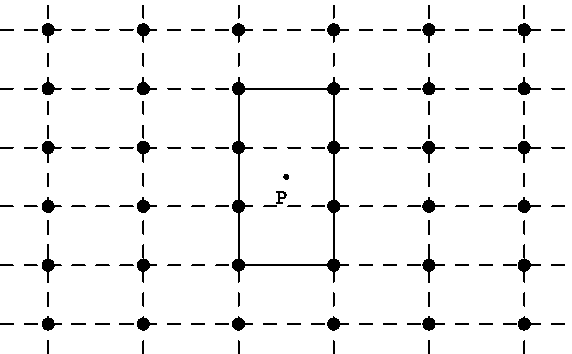
\includegraphics[width=0.5\textwidth]{GuIsLa08cycle2}
	 \caption{A cycle with $|\Group_{C}|=2$}
	 \label{fig:GuIsLa08cycle2}
\end{figure}
%%%%%%%%%%%%%%%%%%%%%%%%%%%%%%%%%%%%%%%%%%%%%%%

The main result in the theory of Ihara zeta functions \refeq{GuIsLa08Zeta}
says that $Z$ is the reciprocal of a holomorphic function, which, up to a
factor, is the determinant of a deformed Laplacian on the graph.


    \PCpost{2016-10-05}{
Unlike in dynamical systems, Ihara zeta functions are defined on
graphs with unoriented (or undirected) edges.

Hashimoto\rf{Hashimoto89}
{\em Zeta functions of finite graphs and representations of p-adic groups}
    }

    \PCpost{2020-05-13}{
Bass\rf{Bass92}
{\em The {Ihara-Selberg} zeta function of a tree lattice}.
It seems that Ihara zeta function walks carry signs - investigate.

He also introduces the \emph{edge zeta function}
to give a determinant form of Ihara zeta function for
undirected graph. This text is from Zhou, Xiao and He\rf{ZhXiHe15},
\arXiv{1502.05771}:

\begin{itemize}
	\item
The \textbf{edge matrix} $W$ of size $[2m \times 2m]$ for an undirected
graph with $m$ undirected edges has entries $w_{ij}$. The $(i,j)$-th
entry of $W$, $w_{ij}$, is a complex variable if the edge $e_i$ is
connected with edge $e_j$ with $e_j \neq e_i^{-1}$, and the entry is 0 if
otherwise.
	\item
For a closed path $C$ in an undirected graph $X$ written as a sequence of
edges $C = e_1e_2 \cdots e_s$, the \textbf{edge norm} of $C$ is
	\[N_E(C) = w_{12}w_{23} \cdots w_{s1}.\]
\end{itemize}
The edge zeta function is defined as follows
\[\zeta_E(W,X) = \prod_{[P] \in \rm{Prime \ Cycles}} (1-N_E(C))^{-1}. \]
It is clear from this definition that if $w_{ij}$ is set to $z \in
\mathbb{C}$, we recover the original Ihara zeta function such that
\[\zeta_G(z) = \zeta_E(W_1,G),\]
where $W_1$ is the edge matrix when all non-zero entries set to $z$.

Furthermore, we have the following formula (cf. Chapter 3 of
Terras\rf{Terras10})
\beq
\zeta_E(W,G) = {\rm Det}(I - W)^{-1}
\,.
\ee{ZhXiHe15:edge_zeta}
    }


    \PCpost{2016-10-05}{
In {\em A Window Into Zeta and Modular Physics}\rf{KirWil10} (that should
warm Li Han's heart) Audrey Terras discusses
\HREF{http://library.msri.org/books/Book57/files/30terras.pdf} {Ihara
zeta function}. She says: ``the Ruelle zeta function of a dynamical
system, will be shown to be a generalization of the Ihara zeta.'' Things
are looking deep. ``It  turns  out  (using  the Ihara  determinant
formula  again)  that  the  Riemann hypothesis means that the graph is
Ramanujan'', etc. She also discusses it in \refref{Terras10} {\em Zeta
Functions of Graphs: A Stroll through the Garden}.

To swoon over the multitude of zetas, read Bartholdi\rf{Bartholdi14} {\em
{Zeta} functions of graphs: a stroll through the garden, by {Audrey
Terras}\rf{Terras10}. Book review}.

Teimoori Faal and M. Loebl\rf{TeiLoe12}
{Bass' identity and a coin arrangements lemma}

Like my \tzeta s,
\HREF{http://kam.mff.cuni.cz/~loebl/clanky/corsica.pdf}{Loebl}'s
Ihara-Selberg function of $G$ is  the infinite product is over the set of
the prime reduced cycles of $G$.

Loebland and Somberg\rf{LoeSom15}
{\em Discrete {Dirac} operators, critical embeddings and {Ihara-Selberg} functions}

da Costa\rf{daCosta16}
{\em The {Feynman} identity for planar graphs}: ``
The Feynman identity (FI) of a planar graph relates the Euler polynomial
of the graph to an infinite product over the equivalence classes of
closed nonperiodic signed cycles in the graph. The main objectives of
this paper are to compute the number of equivalence classes of
nonperiodic cycles of given length and sign in a planar graph and to
interpret the data encoded by the FI in the context of free Lie
superalgebras. This solves in the case of planar graphs a problem first
raised by Sherman and sets the FI as the denominator identity of a free
Lie superalgebra generated from a graph. Other results are obtained
on the zeta functions of graphs.
''

da Costa
{\em Graphs and Generalized Witt identities}
\arXiv{1409.5767}
}

    \PCpost{2016-10-05}{
Sato\rf{Sato05}
{\em Bartholdi zeta functions of group coverings of digraphs}:

The (Ihara) zeta function of a graph G is defined\rf{Ihara66} to be a function of
with u sufficiently small, by
\beq
  Z(G,u)=Z_G(u)=\prod_{[C]}\frac{1}{1-u^{[C]}}
\,,
\ee{Sato05Zeta}
where $[C]$ runs over all equivalence classes
of prime, reduced cycles of G.

 Samuel Cooper and Stratos Prassidis (2010) {\em Zeta functions of infinite
 graph bundles}, % Linear and Multilinear Algebra, 58:2, 185-201,
\HREF{https://doi.org/10.1080/03081080801928084} {DOI} :\\
Originally, Ihara defined the zeta function on finite graphs imitating
the classical definition of the zeta function, where the product is over
all equivalence classes of primitive closed loops C, and $[C]$ denotes
the length of $C$.
    }

    \PCpost{2016-10-05}{
Horton\rf{Horton07}
{\em Ihara zeta functions of digraphs}
considers digraphs whose adjacency matrices are directed edge matrices.

Tarfulea and Perlis\rf{TarPer09}
{An {Ihara} formula for partially directed graphs}: ``
In 2001 Mizuno and Sato showed that the Ihara zeta function of a fully
directed graph has a similar expression, and in 2005, Sato\rf{Sato05} generalized
Ihara's formula to connected, simple, partially directed graphs. (Sato
proved his formula for the more-general two-variable Bartholdi zeta
function.) This paper provides a new proof of Ihara's formula for the
Ihara zeta function of any finite graph, not necessarily connected or
simple, no matter whether it is undirected, fully directed, or partially
directed.
''
    }

    \PCpost{2016-10-30}{
I worry a lot about what time-reversibility means - {\catlatt} is both
time and space reversible, and then there are Ihara zeta functions for
undirected graphs. So I find this interesting: Coppersmith, Kadanoff and
Zhang\rf{CopKadZha01} {\em Reversible {Boolean} networks {I:} distribution of
cycle lengths}. They write: ``
We [...] consider time-reversible dynamics of N Boolean variables models,
with the time evolution of each depending on K of the other variables, which
necessarily have the property that every possible point in the state space is
an element of one and only one cycle. The orbits can be classified by their
behavior under time reversal. The orbits that transform into themselves under
time reversal have properties quite different from those that do not; in
particular, a significant fraction of latter-type orbits have lengths
enormously longer than orbits that are time-reversal symmetric. For large K
and moderate N, the vast majority of points in the state space are on one of
the time-reversal singlet orbits. However, for any finite K, the random
hopping approximation fails qualitatively when N is large enough (N>22K).
When K is large, typical orbit lengths grow exponentially with N, whereas for
small enough K, typical orbit lengths grow much more slowly with N. The
numerical data are consistent with the existence of a phase transition at
which the average orbit length grows as a power of N at a value of K between
1.4 and 1.7. However, in the reversible models, the interplay between the
discrete symmetry and quenched randomness can lead to enormous fluctuations
of orbit lengths and other interesting features that are unique to the
reversible case.
''

Need to check also

Toffoli and Margolus\rf{TofMar90}
{\em Invertible cellular automata: {A} review}

D'Souza and Margolus\rf{SouMar99} {\em Thermodynamically
reversible generalization of diffusion limited aggregation}

}

\item[2020-05-11 Predrag]
Deitmar\rf{Deitmar15} {\em Ihara zeta functions of infinite weighted
graphs}: ``The theory of Ihara zeta functions is extended to infinite
graphs which are weighted and of finite total weight. In this case one
gets meromorphic instead of rational functions and the classical
determinant formulas of Bass and Ihara hold true with Fredholm
determinants.''

\HREF{https://scholar.google.com/citations?hl=en&user=P74k94cAAAAJ}
{Tempesta}\rf{Tempesta15}
{\em A theorem on the existence of trace-form generalized entropies}

Tempesta\rf{Tempesta16} {\em Beyond the {Shannon-Khinchin} formulation:
{The} composability axiom and the universal-group entropy}

\item[2020-05-11 Predrag]
Supriyo Dutta and Partha Guha
{\em Ihara Zeta Entropy},\\
\arXiv{1906.02514};
%Supriyo Dutta and Partha Guha
{\em A System of Billiard and Its Application to Information-Theoretic Entropy},
\arXiv{2004.03444}:
they define Ihara entropy,
an information-theoretic entropy based on the Ihara zeta function of
a graph. A dynamical system consists
of a billiard ball and a set of reflectors correspond to a combinatorial
graph.  The reflectors are represented by the vertices of the graph.
Movement of the billiard ball between two reflectors is represented by the
edges.  The prime cycles of this graph generate the bi-infinite
sequences of the corresponding symbolic dynamical system.  The number
of different prime cycles of a given length can be expressed in terms of
the adjacency matrix of the oriented line graph.  It also constructs the
formal power  series  expansion  of Ihara zeta function.  Therefore,  the
Ihara entropy has a deep connection with the dynamical system of
billiards.

\item[2017-03-08 Predrag]
Reading Band, Harrison and Joyner\rf{BHJ12}
{\em Finite pseudo orbit expansions for spectral quantities of quantum graphs}
one expects to run into another rediscovery of Ihara zeta functions, as the
links are not directed:

``
The \emph{quantum graphs} we consider are metric graphs equipped with a self-adjoint
differential operator $\mathcal{H}$, the Hamiltonian.
Here we are particularly interested in the negative Laplace operator,
\begin{equation}
\mathcal{H}\ :\ f(x)\mapsto-\frac{d^{2}f}{dx^{2}} \ , \label{E:lap_op}
\end{equation}
 or the more general Schr\"odinger operator,
\begin{equation}
\mathcal{H}\ :\ f(x)\mapsto-\frac{d^{2}f}{dx^{2}}+V(x)f(x) \ ,\label{E:schrod}
\end{equation}
 where $V(x)$ is a \emph{potential}, which we assume to be bounded
and piecewise continuous. Note that the value of a function or the
second derivative of a function at a point on the bond is well-defined,
thus it is not important which coordinate, $x_{b}$ or $x_{\hat{b}}$
is used. This is in contrast to the first derivative which changes
sign according to the direction of the chosen coordinate.
''

Indeed, they go through the usual steps of defining oriented graphs and then
putting pairs of oriented bonds on each link, etc. This is explored further
in

Ren, Aleksi{\'{c}}, Emms, Wilson and Hancock\rf{RAEWH10}
{\em Quantum walks, {Ihara} zeta functions and cospectrality in regular graphs}:
review the literature on the discrete-time quantum walks and the Ihara
zeta function.

Setyadi and Stor\rf{SetSto13}
 {\em Enumeration of graphs with the same {Ihara} zeta function}

Higuchi, Konno, Sato and Segawa\rf{HKSS14}
{\em A remark on zeta functions of finite graphs via quantum walks}

Saito\rf{Saito18} {\em A proof of {Terras}' conjecture on the radius of
convergence of the {Ihara} zeta function}
has a nice explicit matrix example, and eigenvalues computation.


    \PCpost{2020-05-05}{
Mizuno and Sato\rf{MizSat01} {\em Zeta functions of digraphs} define a
zeta function of a digraph and an L-function of a symmetric digraph. That
is the usual Bowen-Ruelle (in ChaosBook topological) zeta function.
Tarfulea and Perlis\rf{TarPer09} do note:
``The formula for the zeta function of a directed graph was proved in
1968, wearing a thin disguise, by Bowen and Lanford\rf{BowLan70}. The
elementary connection to directed graphs is made explicit in Th.6.4.6 of
Lind Marcus\rf{LindMar95}.''

Various authors, such as Zhou, Xiao and He\rf{ZhXiHe15} {\em Seiberg
duality, quiver gauge theories, and {Ihara}'s zeta function},
nevertheless refer to it as ``Ihara'', see their Table~2 {\em Ihara zeta
functions for various toric phases of del Pezzo and Hirzebruch quivers}.
Apparently, ``the toric phases are the most popular.''

``The coefficients of the inverse of Ihara zeta function are related to
simple cycles.  In gauge theories, this translates to generic
super-potentials that can be generated from certain quivers.''
This seems to be expansion of a topological zeta function in
terms of fundamental cycles.
    }

    \PCpost{2020-05-05}{
Davey, Hanany and Pasukonis\rf{DaHaPa10}
{\em On the classification of brane tilings}, \arXiv{0909.2868}.
(See also \arXiv{hep-th/0503149}) has an Appendix~A {\em Tiling catalog}.

A brane tiling (or dimer model) is a periodic bipartite graph on the
plane.  Alternatively, we may draw it on the surface of a 2-torus by
taking the smallest repeating structure(known as the fundamental domain)
and identifying opposite edges [1].  The bipartite na-ture of the graph
allows us to colour the nodes either white or black such that white nodes
only connect to black nodes and vice versa.
    }

    \PCpost{2020-05-05}{
Sunada\rf{Sunada13} {\em Topological Crystallography}.
Have the book \CBlibrary{Sunada13}, but do not know how to get useful
info for \catlatt\ out of it.

``the Ihara zeta function [is] a graph-theoretic analogue of class field
theory, discrete Laplacians, and harmonic maps.''

Again, ``Abel–Jacobi maps'' pop up, and again I have no idea what they
are.

    }

    \PCpost{2020-05-06}{
Ren, Wilson and Hancock\rf{ReWiHa11}
{\em Graph characterization via {Ihara} coefficients}:
For an unweighted graph, the Ihara zeta function is the reciprocal of a
quasi characteristic polynomial of the adjacency matrix of the associated
oriented line graph.

First, we demonstrate how to characterize unweighted graphs in a
per\,mut\,ation-invariant manner using the polynomial coefficients from the
Ihara zeta function, i.e., the Ihara coefficients.

Second, we generalize the definition of the Ihara coefficients to
edge-weighted graphs, using the reduced Bartholdi zeta function.

Experimental results reveal that the Ihara coefficients are more
effective than methods based on Laplacian spectra.

Bul{\`{o}}, Hancock, Aziz and Pelillo\rf{BHAP12} {\em Efficient
computation of {Ihara} coefficients using the {Bell} polynomial
recursion}:
They present a method for computing the Ihara coefficients in terms of
complete Bell polynomials and show how the Ihara coefficients can be
efficiently computed provided that the eigenvalues of the adjacency
matrix are known.
}

\item[2020-05-05 Predrag]
Arrigo,
\HREF{https://scholar.google.com/citations?hl=en&user=CKmGEiwAAAAJ}
{Grindrod},  Higham and Noferini\rf{AGHN18}
{\em On the exponential generating function for non-backtracking walks}
do not mention ``Ihara", but seem to derive it anyway from a 3-term recurrence
relation. They write:


We derive an explicit formula for the exponential generating function
associated with non-backtracking walks around both
undirected and directed graphs. Eliminating backtracking
walks in this context does not significantly increase the computational
expense. We show how the new measures may be interpreted in terms of
standard exponential centrality computation on a certain multilayer
network. Insights from this block matrix interpretation also allow us to
characterize centrality measures arising from general matrix functions.

\item[2020-05-11 Predrag]
Bharatram Rangarajan
{\em A combinatorial proof of Bass's determinant formula for the zeta
function of regular graphs}, \arXiv{1706.00851}:
The zeros and poles of the Selberg zeta
function appear in the Selberg trace formula, which relates the
distribution of primes with the spectrum of the Laplace-Beltrami operator
of the surface. The idea of considering closed geodesics as primes
inspired the work of Hashimoto\rf{Hashimoto89}, Bass\rf{Bass92}, Kotani
and Sunada\rf{KotSun00} to come up with an analogous notion in the
discrete setting.

Just like the Selberg zeta function is related to the spectrum of the
Laplace-Beltrami operator of the surface, it is natural to ask if its
discrete analogue, the Ihara zeta function of a graph, is related to the
spectrum of the Laplacian matrix (or the adjacency matrix) of the graph.
Bass\rf{Bass92} gives an expression for the Ihara zeta function of a
graph $G=(V,E)$ as
$$
\zeta_G(t) = \frac{1}{(1-t^2)^{|E|-|V|} \det(I-tA+(D-I)t^2)}
$$
where $A$ is the adjacency matrix of $G$ and $D$ is the diagonal matrix
of degrees of the vertices of $G$, or in other words, $D=diag(A\vec{1})$.
In particular, if $G$ is $d$-regular, then (see \refeq{GridAdjec},
derivation \refeq{Rangarajan2a})
\beq
\zeta_G(t) = \frac{1}{(1-t^2)^{|E|-|V|} \det(I-tA+(d-1)t^2I)}
\ee{Rangarajan2}
gives a way of obtaining the set of poles
of $\zeta_G(t)$.

For a general, partially directed graph see Sato\rf{Sato05} and
Tarfulea and R. Perlis\rf{TarPer09}.

Most proofs Bass's determinant formula start by expressing the zeta
function in terms of not the adjacency matrix $A$ of $G$, but the
adjacency matrix $H$ of the oriented line graph of $G$ (called the
Hashimoto edge-incidence matrix).

In this paper, we shall see a more elementary combinatorial proof of
Bass's determinant formula in the case when $G$ is regular.
The proof goes as
follows:
\begin{itemize}
\item
    The zeta function $\zeta_G({z})$ has an expansion of the form
$$
\zeta_G({z})= \exp\left( \sum \limits_{k=1}^{\infty} N_k \frac{{z}^k}{k} \right)
$$
where for $k \in \integers$, $N_k$ is the number of rooted,
\emph{non-backtracking} cycles in $G$ of length $k$.
\item
    An expression for $N_k$ is not immediate, the starting
    point is the study of non-backtracking walks on $G$. We can construct
    the family $\{A_k\}_{k \in \mathbb{Z}_{\small{\geq 0}}}$ of $n \times
    n$ matrices such that for every $k \in \mathbb{Z}_{\small{\geq0}}$
    and every $v,w \in V$, $(A_k)_{vw}$ is the number of
    non-backtracking walks on $G$ of length $k$ from $v$ to $w$.
\item
    $N_k$ is combinatorially computable from $\Tr(A_k)$.
\item
    $\Tr(A_k)$ is well-understood in terms of the eigenvalues of $A$ and
    a family of Chebyshev polynomials. These ingredients lead to a proof
    of Bass's determinant formula.
\end{itemize}


%\section{Non-backtracking walks and Chebyshev polynomials}
$(A^k)_{vw}$ counts the total number of walks (with backtrackings) on $G$
from $v$ to $w$ of length $k$. Let
$$A_0,A_1,A_2,A_3,\dots$$
be $[n \times n]$ matrices over $\complex$ such that the value $(A_k)_{vw}$
is the number of \emph{non-backtracking} walks on $G$ from $v$ to $w$ of length
$k$. This family $\{A_k\}_{k \in \integers}$ can be recursively defined
using powers of $A$ as follows:
\begin{itemize}
\item $A_0=I$
\item $A_1=A$
\item $A_2=A^2-dI$
\item For $k \geq 3$,
$$A_k=A\,A_{k-1}-(d-1)A_{k-2}$$
\end{itemize}
This recurrence relation shows that the
ordinary (matrix) generating function for the above sequence is
$$\sum \limits_{k=0}^{\infty} {z}^k A_k = (1- {z}^2)I.
  \left( I-{z}A + (d-1){z}^2 I \right)^{-1}$$
\ie, generating function
$$\frac{1-{z}^2}{1-A{z}+(d-1){z}^2}$$

Consider the
family of Chebyshev polynomials of the second kind
$$U_0(x), U_1(x), U_2(x), \dots $$
defined by the recurrence
$$U_0(x)=1$$
$$U_1(x) = 2x$$
and for $k \geq 2$,
$$U_k(x) = U_{k-1}(x)U_1(x) - U_{k-2}(x)$$
and with generating function
$$\sum \limits_{k=0}^{\infty} U_k(x){z}^k = \frac{1}{1-2x{z}+{z}^2}$$

It is easy to see that
$$\sum \limits_{0 \leq j \leq k/2} A_{k-2j} = (d-1)^{k/2} U_k \left( \frac{A}{2\sqrt{d-1}} \right)$$
implying that for $k \geq 2$,
$$A_k = (d-1)^{k/2} U_k \left( \frac{A}{2 \sqrt{d-1}} \right)
      - (d-1)^{k/2-1} U_{k-2} \left( \frac{A}{2 \sqrt{d-1}} \right)$$
This holds for $0 \leq k \leq 2$ as well, if
$$U_m(x) = 0$$
for every $m < 0$. This allows us to work with the above expression for
$A_k$ for \emph{all} non-negative integers $k$.

Taking trace on both
sides,
$$
\Tr(A_k) = (d-1)^{k/2} \sum \limits_{j=0}^{n-1}
             U_k \left( \frac{\mu_i}{2 \sqrt{d-1}} \right)
         -(d-1)^{k/2-1} \sum \limits_{i=0}^{n-1}
             U_{k-2} \left( \frac{\mu_i}{2 \sqrt{d-1}} \right) $$
where
$$d=\mu_0 \geq \mu_1 \geq \dots \geq \mu_{n-1} \geq d$$
are the $n$ eigenvalues of the adjacency matrix $A$. Thus we have an
expression for the trace of $A_k$ as a polynomial in the eigenvalues of
$A$.
% This approach is used in the seminal work of Lubotzky, Phillips and
% Sarnak in their construction of Ramanujan graphs. % \cite{lps},
For a detailed and elementary exposition of Chebyshev polynomials and
non-backtracking walks on regular graphs, the reader is referred to the
monograph by Davidoff, Sarnak and Valette\rf{DaSaVa03}.

While $(A_k)_{vw}$ counts the number of walks on $G$ from vertex $v$ to
vertex $w$ without backtracking, the diagonal element
$(A_k)_{vv}$ does \emph{not} count the number of non-backtracking cycles
of length $k$ rooted at $v$. This is because $(A_k)_{vv}$ also counts
walks of the form
$$e_1 e_2 \dots e_k$$
where $e_{i+1} \neq \overline{e_i}$ for any $1 \leq i \leq k-1$ but
$e_k = \overline{e_1}$. That is, $e_1 e_2 \dots e_k$ is non-backtracking
as a walk from $v$ to $v$, but when considered as a closed walk (or a
loop), the two end edges form a backtracking! Such an instance of a
backtracking that gets overlooked in $\Tr(A_k)$ shall be referred to as a
\emph{tail}.

So $\Tr(A_k)$ counts the number of closed, rooted walks
of length $k$ that could have at most $1$ tail, and hence does \emph{not}
count the  rooted, non-backtracking cycles of length $k$. It is
interesting to ask what the number of closed, rooted non-backtracking
walks of length $k$ is.

Relation between $M_k=\Tr(A_k)$ and $N_k$:
For every $k \geq 3$,
$$N_k = \begin{cases}
M_k - (d-2) (M_{k-2}+M_{k-4}+\dots+M_1) & \text{ odd   }k \\
M_k - (d-2) (M_{k-2}+M_{k-4}+\dots+M_2) & \text{ even }k
\end{cases}$$
By linearity of trace,
$$N_k=\begin{cases}
\Tr\left( A_k - (d-2)(A_{k-2}+A_{k-4}+\dots+A_1) \right) & \text{ if k is odd}\\
\Tr\left( A_k - (d-2)(A_{k-2}+A_{k-4}+\dots+A_2) \right) & \text{ if k is even}\\
\end{cases}$$
[... after a few steps ... this is related to]
$$U_k(x) - U_{k-2}(x) = 2 T_k(x)$$
where $T_k(x)$ is the \emph{Chebyshev polynomial of the first kind}
defined by
\bea
T_0(x) &=& 1\,,\quad
T_1(x)=x
    \continue
T_k(x)  &=&  2x T_{k-1}(x) - T_{k-2}(x)
\quad \mbox{for } k \geq 2
\,,
\label{Rangarajan17:TkRecurr}
\eea
with the generating function
\beq
\sum \limits_{k=0}^{\infty} T_k(x)z^k = \frac{1-xz}{1-2xz+z^2}
\ee{Rangarajan17:TkGenFunct}
[... after a few probably unnecessary steps, ... taking a derivative ...
this is related to]
\begin{align}
N_1{z} + & N_2 \frac{{z}^2}{2} + N_3 \frac{{z}^3}{3} + \dots \\
& = -\frac{n(d-2)}{2} \ln{(1-{z}^2)}
    - \sum \limits_{j=0}^{n-1} \ln{(1-\mu_j {z} + (d-1){z}^2)} \\
& = -\left( \frac{nd}{2} - n \right) \ln{(1-{z}^2)}
    - \ln{\left( \prod \limits_{j=0}^{n-1}1-\mu_j {z} + (d-1){z}^2 \right) }\\
& = -(|E|-|V|) \ln{(1-{z}^2)} - \ln{ \left(\det(I-A{z}+(d-1){z}^2) \right)}
\label{Rangarajan17:templattGenFct}
\end{align}
resulting in \refeq{IharaTheo}:
\\
%\begin{theorem}[Bass's determinant formula]
{\bf Bass's determinant formula}
Let $G=(V,E)$ be a $d$-regular graph with adjacency matrix $A$, and let
$N_k$ count the number of rooted, non-backtracking cycles of length $k$
in $G$. Then
\beq
\zeta_G({z}) = \frac{1}{(1-{z}^2)^{|E|-|V|} \det(I-{z}A+(d-1){z}^2I)}
\ee{Rangarajan2a}
%\end{theorem}









\end{description}

\subsection{Maillard}
\label{sect:Maillard}

Another scary line of literature. Connecting Baxter to dynamical zetas
functions. Maillardinians have a burst at the end of 20th century. Very easy
to collect the literature, as only they cite their own articles, and nobody
else cites them.

A cute cat map exercise - but I have to bike home, will continue
later...

\begin{description}

    \item[2016-11-16 Predrag]
Angl{\`e}s d'Auriac, Boukraa and Maillard\rf{AnBoMa99}
{\em Functional relations in lattice statistical mechanics, enumerative
combinatorics, and discrete dynamical systems} write `` ... non-linear
functional relations appearing in [...] lattice statistical mechanics [...]
We then consider discrete dynamical systems corresponding to birational
transformations. The rational expressions for dynamical zeta functions
obtained for a particular two-dimensional birational mapping, depending on
two parameters [...] compatible with a chaotic dynamical system.

They obsess about the Arnol'd complexity, which counts the number of
intersections between a fixed line  and its $n$th iterate. I do not see why
we should care.

I like Bedford and Diller\rf{BedDil05} {\em Real and complex dynamics of a
family of birational maps of the plane: {The} golden mean subshift} better,
so I follow their notation here. It's a rather impressive paper.

For reasons known to some people (symmetries of Baxter models?) they study a
birational transformation and its inverse,
\bea
\begin{array}{ccl}
 x_{n+1} &=& y_n\,\frac{x_n + a}{x_n - 1}         \\
 y_{n+1} &=& x_n + a - 1
\end{array}
    \qquad
\begin{array}{ccl}
 x_{n-1} &=& y_n + 1-a    \\
 y_{n-1} &=& x_n\,\frac{y_n - aa}{y_n + 1}
\end{array}
\,,\qquad a\in\reals
\,.
\label{eq:AABHM99-3}
\eea
The map is area-preserving in the sense that it preserves a meromorphic
2-form
\[
\frac{dx\wedge dy}{y-x+1}
\]
and is reversible, which means that the map is conjugate to its
inverse via involution $(x,y)\to(-y,-x)$.
The inverse transformation amounts to $y_n\leftrightarrow -z_n$, \ie, the
time reversal symmetry, and the $x-y=0$ line is the \emph{time-reversal
invariant line}.
The {\tzeta} for \refeq{eq:AABHM99-3} is
\beq
\zetatop(z) =  \frac{1 - z - z^2}
                    {1 - z^2}
 \,.
\ee{AABHM99-28}
It counts all \po s, real and complex.
Interestingly, this zeta satisfies an elegant functional relation
relating $\zeta(z)$ and $\zeta(1/z)$.

The zeta function for real roots is complicated and depends on the parameter
$a$.

                                        \toCB
Bedford and Diller\rf{BedDil05} construct a generating partition and the
Markov diagram (they call that Graph of Filtration), including the transient
nodes. The recurrent part of this graph is just the golden mean graph, with
11 repeats forbidden. They obsess much about their ``rectangles.'' Show that
all \po s are hyperbolic. Discuss pre-periodic orbits. Zeta functions are
never mentioned, though topological entropy is computed.

Abarenkova \etal\rf{AABHM99} {\em Rational dynamical zeta functions for
birational transformations} is not worth reading - the material is better
explained in their other papers.

If the dynamical zeta function can be interpreted as the ratio of two
characteristic polynomials of two linear operators  $A$ and $B$, namely
\beq
\frac{1}{\zeta(z)}=\frac{\det(1-zA)}{\det(1-zB)}
\,,
\ee{AABHM99-56a}
then the number of fixed points is given by
\beq
\Tr(A^n)-\Tr(B^n)
\,.
\ee{AABHM99-56b}
In this linear
operators framework, the rationality of the $\zeta$
function\rf{Guckenheimer70,manning}, and therefore the algebraicity of the
exponential of the topological entropy, amounts to having a finite dimensional
representation of the linear operators $A$ and $B$.

Their only explicit example of a rational zeta dynamical
function is the case of the Arnol'd cat map on torus
\(\mathbb{T}^2 =  \reals^2/\integers^2\,,\)
\beq
 {A} =\left(\begin{array}{cc}
 2 & 1 \\
 1 & 1
  \end{array} \right)
\,,\qquad
 {B} =\left(\begin{array}{cc}
 1 & 0 \\
 0 & 1
  \end{array} \right)
\ee{AABHM99-56c}
The {\tzeta}\rf{Isola90} for Arnol'd cat map is
\beq
\zetatop(z)
    = \frac{\det(1-zA)}{\det(1-zB)}
    =  \frac{1 - 3 z + z^2}
                  {(1 - z)^2}
 \,.
\ee{AABHM99-56d}

    \item[2016-06-02, 2020-09-24 Predrag]
From my notes on Isola\rf{Isola90}
{\em {$\zeta$}-functions and distribution of periodic orbits of toral automorphisms},
see \refsect{sect:Isola90}: [...]
The {\tzeta} for cat-map class of models is (see \refeq{AABHM99-46})
\beq
\zetatop(z) % = \frac{(1 - \Lambda z) (1 - \Lambda^{-1} z)}
            %        {(1 - z)^2}
           =  \frac{1 - s z + z^2}
                  {(1 - z)^2}
 \,.
\ee{Ising:Isola90-13}
Define
\beq
d(s)
= {z^{-1} - {s} + z}
\ee{detCat}
then (compare with \refeq{AABHM99-56a})
\beq
  \zetatop(z)
  = \frac{d(s)}{d(2)}
  = 1+\frac{d(s)-d(2)}{d(2)}
  = 1 - {\mu}^2\frac{1}{d(2)}
\ee{zetaCat}

I wonder whether the fact that this is quadratic in $z$ has something to do
with the time-reversibility, and the unsigned graph's Ihara zeta functions?

The ``characteristic function''  \refeq{FGHLW74:charFunct1d}
for the 3-point recurrence centered on the $s$ term, $1/z-s+z$ suggests
multiplying \refeq{Ising:Isola90-13} by $z^{-1}/z^{-1}$. That leads to
\beq
\zetatop(z) = 1 + \frac{{\mu}^2}
                  {(1 - z)(1 -1/z)}
           =  1 + \left(
                   \frac{z}{1 - z} + \frac{1/z}{1 - 1/z}
                  \right){\mu}^2
\,.
\ee{IIsola90-13d}
Interpretation: the \templatt\ zeta function denominator is
the Laplacian, and ${\mu}^2$ is measuring the deviation from the pure Laplacian
case (marginal, no solutions other than the $n=1$ (line of) fixed point(s).

Conversely, given the \tzeta, the generating
function for the number of temporal {\lattstate}s of period $\cl{}$ is
given by the logarithmic derivative of the {\tzeta} \refeq{zetatop-N},
\bea
\sum_{{n}=0}^\infty N_{n} z^{n}
    & = & \frac{2-{s}z}{1 - s z + z^2}-\frac{2}{1 - z}
      =   \frac{2/z-{s}}{1/z - s + z}-\frac{2}{1 - z}
    \continue
& = & \frac{(2/z-{s})(1 - z)-2(1/z - s + z)}{(1/z - s + z)(1 - z)}
    \continue
& = & {\mu}^2\frac{1+z}{(1/z - s + z)(1 - z)}
    \continue
& = & {\mu}^2\left[z + ({s}+2) z^2 + ({s}+1)^2 z^3 \right.
    \ceq
      \left.\qquad\quad
      +\,({s}+2)\,{s}^2 z^4 + (s^2+ s-1)^2 z^5  +  \cdots\right]
\,.
\label{1stChebGenF}
\eea
which is indeed the generating function for $T_{\period{}}(s/2)$, the
Chebyshev polynomial of the first kind.
% of \refeq{POsChebyshev}.

To me it looks like we should include (time reflection symmetry!) also
negative $n$ in the $z^n$ series (Laurent series?), with a negative sign,
so I get
\bea
\sum_{{n}=-\infty}^\infty N_{n} z^{n}
    & = & \frac{{\mu}^2}{z^{-1} - s + z}
    \left(\frac{1+z}{1 - z} {\color{red}-} \frac{1+z^{-1}}{1 - z^{-1}}\right)
    \continue
& = & \frac{{\mu}^2}{z^{-1} - s + z}
    \frac{(1+z)(1 - z^{-1}){\color{red}-}(1 - z)(1 + z^{-1})}{(1 - z)(1 - z^{-1})}
    \continue
& = & \frac{2{\mu}^2}{z^{-1} - {\mu}^2-2 + z}\,\frac{z-z^{-1}}{(1 - z)(1 - z^{-1})}
    \continue
& = & \frac{2{\mu}^2}{z^{-1} - {\mu}^2-2 + z}\,\frac{z^{-1}-z}{z^{-1} - 2 + z}
\,.
\label{1stChebGenFa}
\eea

    \item[2020-09-30 Predrag]
The Bernoulli equation rewritten as a first-order
difference equation:
\beq
\ssp_{\zeit} - {s}\ssp_{\zeit-1} = - \Ssym{\zeit}
\,,\qquad  \ssp_{\zeit} \in [0,1)
\,.
\ee{1stepDiffEq}
For a Bernoulli system
\bea
\zetatop(z)
 &=&
\exp \left[\ln(1 -  {s}z) - \ln(1 - z) \right]
\continue
 &=&
\frac{1 -  {s}z}{1 - z}
\,.
\label{BernZeta}
\eea
Define
\beq
d(s)
= {z^{-1} - {s}}
\ee{detBernoulli}
then (compare with \refeq{AABHM99-56a})
\beq
  \zetatop(z) = \frac{d(s)}{d(2)}
  = 1+\frac{d(s)-d(2)}{d(2)}
  = 1+ (s-1)\frac{1}{d(2)}
\ee{zetaBernoulli}
The numerator $(1 - {s}z)$ says that a Bernoulli system is a full
shift\rf{CBcount}: there are $s$ fundamental {\lattstate}s and every
other {\lattstate} is built from their concatenations and repeats.

    \item[2020-09-24 Predrag]
For 2\dmn\ \catlatt\ the ``characteristic function''
\refeq{FGHLW74:charFunct1d} the above musings suggests a guess
\bea
\zetatop(z_1,z_2)
&=&
 \frac{z_1 + z_2 - 2{s} + z_1^{-1} + z_2^{-1}}
      {z_1 + z_2 -   4  + z_1^{-1} + z_2^{-1}}
\continue
&=&
1 -
 \frac{2{\mu}^2}
      {z_1 + z_2 -   4  + z_1^{-1} + z_2^{-1}}
\label{PCcatLattZeta1}\\
&=& 1 +
 \frac{2{\mu}^2}
      {(1 - z_1)(1 -1/z_1)+(1 - z_2)(1 -1/z_2)}
\nnu
\eea
If we define
\beq
d(s)
= {z_1 + z_2 - 2{s} + z_1^{-1} + z_2^{-1}}
\ee{detCatLatt}
then (compare with \refeq{AABHM99-56a})
\beq
  \zetatop(z_1,z_2) = \frac{d(s)}{d(2)}
\ee{zetaCatLatt}
suggest some derivatives, integrations with respect to the
parameter ${s}$, resulting in $\ln d(s) - \ln d(2)$ from the
ends of the integration domain.

See also \refeq{AABHM99-56d}.

    \PCpost{2020-05-05}{
Kotani and Sunada\rf{KotSun00} {\em Zeta functions of finite graphs}
seems cited a lot and perhaps belongs to \emph{ChaosBook.org}.
    }

    \PCpost{2020-05-05}{
Stark and Terras\rf{StaTer96}
{\em Zeta functions of finite graphs and coverings}
is cited a lot and perhaps belongs to \emph{ChaosBook.org}.

Stark and Terras\rf{StaTer00}
{\em Zeta functions of finite graphs and coverings, {Part II}}

    }



\end{description}

\renewcommand{\Tr}{\mbox{\rm Tr}\,}
%\newcommand{\Tr}{\mbox{Tr}\,}

%followed by
%\section{$X$-$Y$ model}
%\label{sect:XY}
